\chapter{Methodik}
\label{chap:methodik} Dieses Kapitel beschreibt das methodische Vorgehen, das
zur Beantwortung der Forschungsfrage gewählt wurde, um aussagekräftige und reproduzierbare
Ergebnisse zu erzielen. Eine nachvollziehbare Methodik ist essenziell, um die Ergebnisse
sowohl evaluierbar als auch für zukünftige Arbeiten nutzbar zu machen. Das
Hauptziel dieser Arbeit ist die Entwicklung einer stabilen und voll
funktionsfähigen Erweiterung für die Software 3D Slicer, die in der Klinik eingesetzt
werden kann. Zu Beginn wurde demnach eine umfassende Anforderungsanalyse
durchgeführt, um die spezifischen Anforderungen der Domäne zu erfassen und die Ausgangssituation
zu klären. Darauf aufbauend folgte eine detaillierte Literaturrecherche, um den aktuellen
Stand der Technik zu untersuchen und bestehende Lösungen zu identifizieren. Da
das Ziel dieser Arbeit die Entwicklung einer vollständigen Softwarelösung ist, wurde
das Problem anschließend in Teilaufgaben zerlegt. Dies ermöglicht eine gezielte
Bearbeitung einzelner Komponenten und erleichtert die iterative Entwicklung. Falls
für bestimmte Teilbereiche keine passenden Lösungsansätze aus der Literatur ableitbar
waren, wurden darauf basierend eigene Lösungen ‚erarbeitet.

Neben der praktischen Anwendung der entwickelten Erweiterung bietet diese Arbeit
auch wissenschaftlichen Mehrwert. Daher wird im folgenden Abschnitt die gewählte
Methodik detailliert begründet und deren Vorteile herausgearbeitet.
% ---------------------------------------------------------------------------------------

\section{Forschungsdesign}
Das Forschungsdesign dieser Arbeit folgt einem praktischen Entwicklungsansatz mit
einem Fokus auf softwaretechnische Methoden. Zum Erreichen der Ziele stützt sich
diese Arbeit so am Entwicklungsprozess ab und dokumentiert diesen. Dabei lässt sich
der gesamte Zeitraum dieser Arbeit in drei Phasen aufteilen, die jeweils einem
unterschiedlichen Zweck dienen. Diese drei Phasen sollen auch eine grobe Orientierung
bezüglich der Reihenfolge während der Bearbeitung geben.

\pagebreak

\begin{description}
	\item[Analysephase] diese erste Phase ist bei fast allen Softwareprojekten die
		wichtigste Phase und gleichzeitig die, die meist zu kurz kommt. Innerhalb der
		Analysephase werden also alle Anforderungen an die Software gesammelt. Diese
		basieren zum großen Teil auf der Literaturrecherche. Außerdem werden bestehende
		Lösungen analysiert und so die Kernfunktionalität herausgefiltert.

	\item[Entwicklungsphase] die Entwicklungsphase bildet den größten Teil. Hier
		findet die konkrete Umsetzung statt. Hierzu wird das System in mehrere Subsysteme
		unterteilt. Dies ermöglicht eine isolierte Betrachtung. Während der Entwicklung
		wird ein Phototypenansatz verfolgt.

	\item[Evaluationsphase] die letzte Phase dieser Arbeit beschäftigt sich ausschließlich
		mit der Evaluation der Ergebnisse. Hier soll eine Antwort auf die in Kapitel
		\ref{chap:fragestellung} formulierten Fragestellungen gefunden werden.
\end{description}

Durch diese Unterteilung ist eine gutes strukturelles vorgehen Möglich um mittels
einer praktischen Umsetzungsmethodik zu einem guten Ergebnis zu kommen. Die
nächsten Kapitel blicken nun kurz in die einzelnen Phasen, beginnend mit einer Anforderungsanalyse.
% ---------------------------------------------------------------------------------------

\section{Anforderungsanalyse}
\label{sec:anforderungsanalyse} Nach genauerem Betrachten der Fragestellung aus Kapitel
\ref{chap:fragestellung} und den Zielen aus \ref{sec:ziel_der_arbeit} können bereits
erste Anforderungen abgeleitet werden, die für die Erweiterung gelten sollen. Neben
diesen Anforderungen wurden auch die Klinik für Zahnerhaltung mit in diesen Prozess
eingebunden. Hierzu wurde innerhalb einer Besprechung mit dem verantwortlichen
Arzt, Dr. Elias Walter, ein Anforderungskatalog ausgearbeitet \citep[vgl.][]{walter2025}.
Diese Anforderungen waren vor allem zu Beginn der Entwicklung sehr wichtig um einen
ersten Anhaltspunkt zu gewinnen. Im Laufe des Entwicklungsprozesses wurden
Statusberichte eingeplant, die ein Reagieren auf Anforderungsänderungen ermöglichen.

In erster Linie wird klar, dass im Rahme dieser vorliegenden Arbeit eine
Erweiterung für die Plattform 3D Slicer entwickelt werden soll. Die Kernfunktionalität
soll dabei die anatomische Segmentierung bilden, wie sie in Kapitel
\ref{sec:verwwandte_arbeit} beschrieben wurde. Greift man das Ziel dieser Arbeit
aus der Einleitung \ref{sec:ziel_der_arbeit} nochmals auf, dann kann hierdurch
die nächste wichtige Anforderung abgeleitet werden. Die Erweiterung soll gut und
einfach über eine \ac{UI} bedient werden können. Außerdem ist eine stabile Anwendung
gefragt, die sich gut in die Kernanwendung von 3D Slicer einfügt. \citet[]{walter2025}
machte im Interview deutlich, dass die Erweiterung neben einer Einzelbildbearbeitung
auch einen Batch-Prozess ermöglichen so. So können beispielsweise Parameter an
einem Bild erprobt werden und diese anschließend in einen Batch-Prozess auf
viele Bilder überführt werden. Außerdem soll es möglich sein, verschiedenen
Schwellwertverfahren, die in der anatomischen Segmentierung vorgesehen sind,
auch in der Erweiterung auszuwählen. Ein wichtiger Softwaretechnischer Anspruch an
die Extension ist die Erweiterbarkeit. Es soll ohne große Mühen möglich sein, ein
weiteres Verfahren zu integrieren, ohne das große Anpassungen an der UI oder der
Erweiterung selbst unternommen werden müssen. Für ein solides Verständnis dieser
Software soll es selbstverständlich eine Dokumentation mit Benutzerhandbuch geben.
Zudem wird großer Wert auf die Qualitätssicherung gelegt, weshalb eine Reihe von
Unit-Tests (Tests für einzelne Programmeinheiten) vorgesehen ist. Um die
Anforderungen an die Software besser zu verstehen und zu strukturieren, ist neben
der Sammlung technischer Spezifikationen auch ein solides Verständnis für die zugrunde
liegende Domäne essenziell. Die Abbildung \ref{fig:3d_slicer_domäne}
veranschaulicht dies durch ein Domänenmodell, das der \ac{UML} entspricht. Mittels
dieser Grafik, können die gestellten Anforderungen visuell dargestellt werden
\citep[vgl.][]{walter2025}.

\begin{figure}[h]
	\centering
	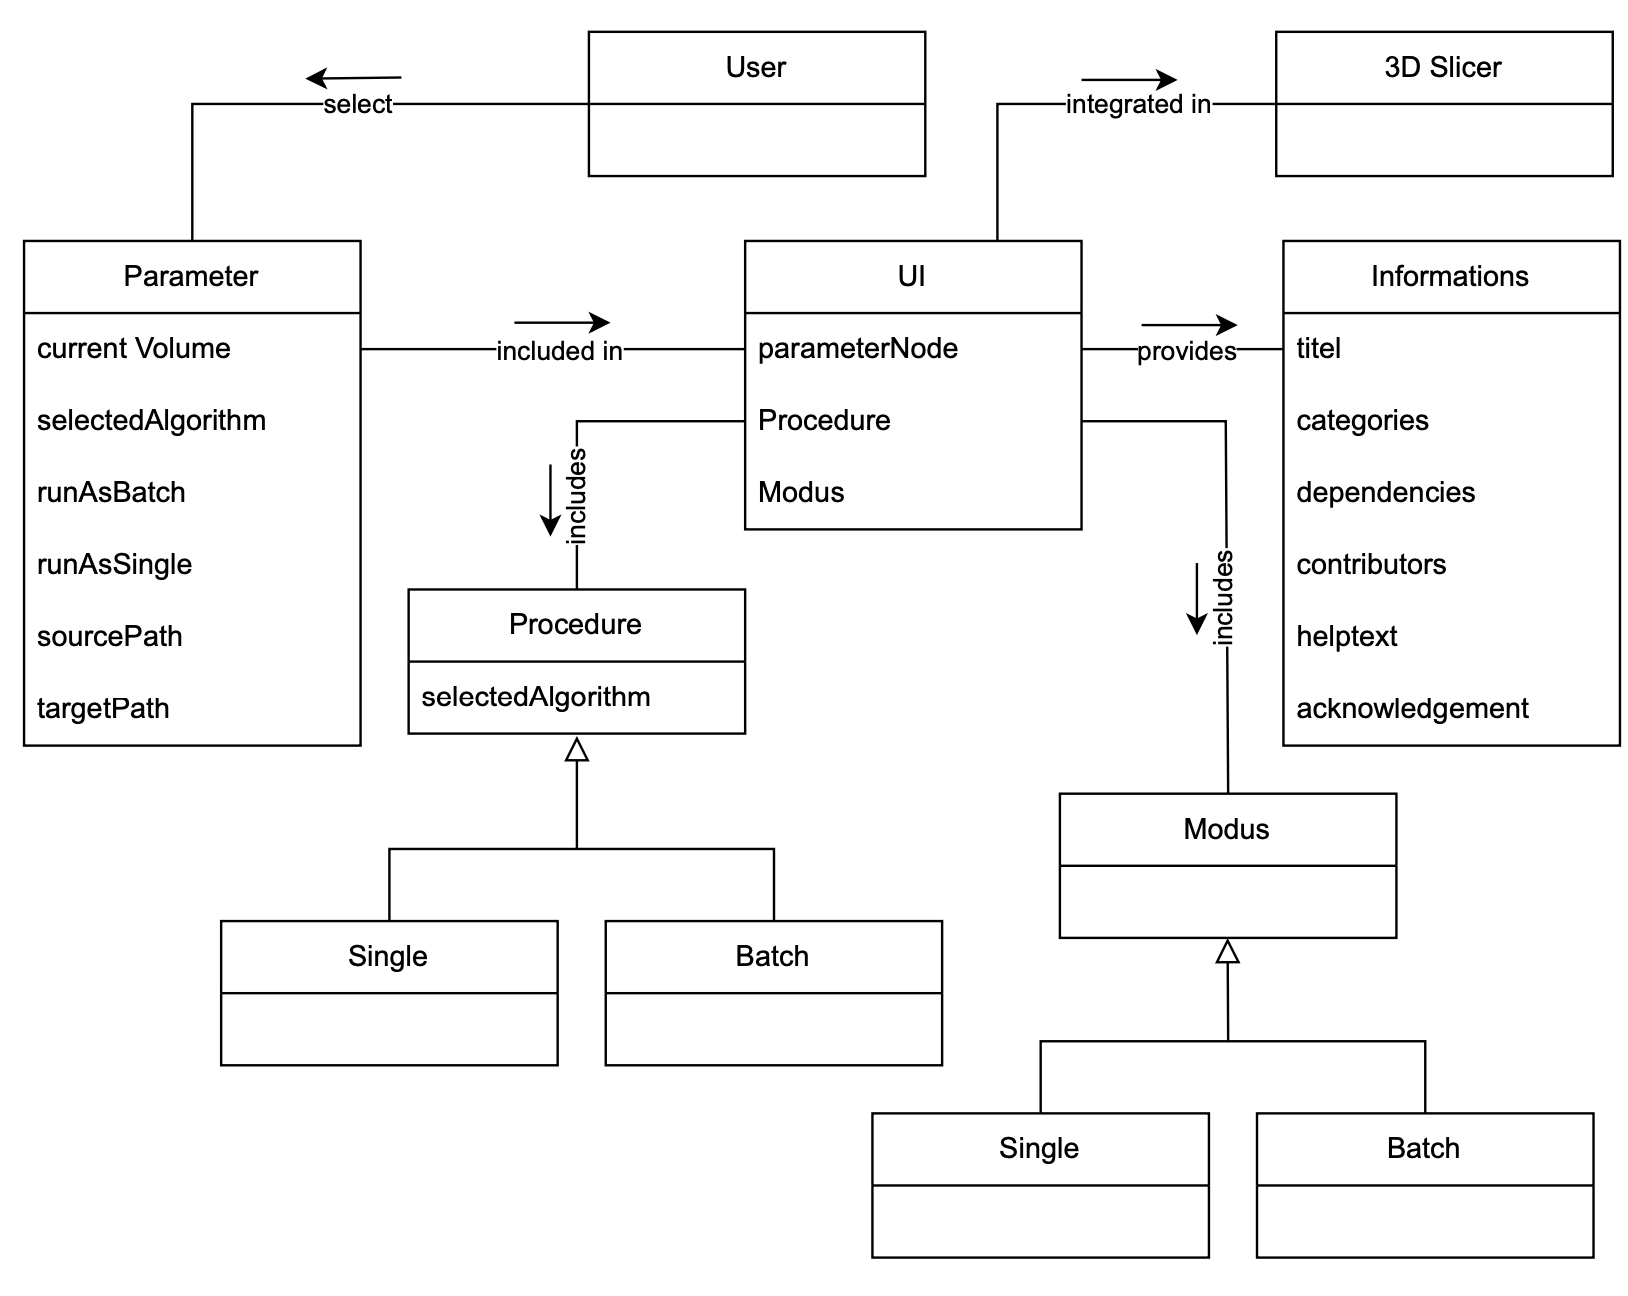
\includegraphics[width=0.75\textwidth]{img/domaenenmodell.jpg}
	\caption{UML-Domänenmodell des gesamten Softwaresystems}
	\label{fig:3d_slicer_domäne}
\end{figure}

Durch diese breite Palette an Anforderungen ergeben sich verschiedene Aufgaben
für die Implementierung. Bevor jedoch mit der konkreten Umsetzung begonnen werden
kann, ist ein noch wichtigerer Schritt erforderlich: die Recherche. Sie dient
dazu, den aktuellen Stand der Technik zu erfassen und geeignete Lösungsansätze zu
identifizieren.
% ---------------------------------------------------------------------------------------

\section{Recherche zum Stand der Kunst}
Es wäre äußerst ungünstig, erst am Ende eines Projekts festzustellen, dass bereits
veröffentlichte Lösungen existieren, in die erhebliche Ressourcen investiert
wurden. Um dies zu vermeiden, ist eine umfassende Literaturrecherche essenziell,
die den aktuellen Stand der Technik abbildet. Dabei wird auf Fachliteratur sowie
domänenspezifische Quellen zurückgegriffen, um alle relevanten Aspekte abzudecken.

Für diese Arbeit spielt eine Quelle eine besonders wichtige Rolle: die
offizielle Dokumentation von 3D Slicer. Sie bietet wertvolle Anhaltspunkte für die
Implementierung und hilft dabei, die technischen Gegebenheiten von 3D Slicer zu
verstehen. Zudem enthält sie \textit{Best-Practice-Ansätze}, die bei der Entwicklung
berücksichtigt wurden. 3D Slicer stellt außerdem einen Developer Guide zur
Verfügung, der Teil der offiziellen Dokumentation ist und den Einstieg in das Framework
erleichtert. Ein weiterer zentraler Referenzpunkt ist der \textit{3D Slicer
Extension Index}, in dem bereits entwickelte Erweiterungen einsehbar sind. Ein konkretes
Beispiel ist das Modul \textit{Airway Segmentation}, dessen Analyse dazu beiträgt,
bewährte Konventionen für die Entwicklung der eigenen Erweiterung abzuleiten. So
kommt es, dass beispielsweise für die Gestaltung einer Benutzerschnittstelle
bereits Lösungen existieren, die sich bewährten und so übernommen werden können.

Neben einer konkreten Implementierungshilfe dient die Literaturrecherche auch dazu,
ein fundiertes Verständnis für die Domäne der medizinischen Bildverarbeitung und
deren zugrunde liegende Strukturen zu entwickeln. Mithilfe verschiedener domänenspezifischer
Publikationen kann ein tieferes Wissen über diesen Fachbereich gewonnen werden.
Besonders relevant sind hierbei die verschiedenen Verfahren für die Verarbeitung
der Mikro-\ac{CT}-Aufnahmen. Konkret handelt es sich hier um die
unterschiedlichen Algorithmen zur Filterung und Segmentierung von Mikro-\ac{CT}-Bildern
in der Zahnmedizin.

Darüber hinaus ermöglicht die Recherche einen Blick auf alternative Plattformen zur
Bildverarbeitung, wie beispielsweise die weit verbreitete Software \ac{ITK-SNAP}.
Ein kurzer Vergleich ergab jedoch, dass diese Lösung aufgrund ihrer Struktur in diesem
speziellen Fall nicht mit 3D Slicer konkurrieren kann.

Die Recherche bietet somit einen ersten fundierten Überblick über mögliche Lösungen
für die einzelnen Anforderungen. Um nun detaillierter auf die Umsetzung
einzugehen, nimmt das nächste Kapitel eine Unterteilung der Gesamtheit der Anforderungen
in kleinere Teilsysteme vor.
% ---------------------------------------------------------------------------------------

\section{Zerlegung in Teilprobleme}
\label{sec_zerlegung_in_teilprobleme} Durch die Aufteilung des Gesamtsystems in mehrere
kleine Teilaufgaben wird die Software für den Entwicklungsphase übersichtlicher.
Die einzelnen Domänen können so schneller und besser verstanden werden. Es gibt viele
Möglichkeiten ein Softwaresystem in kleine Teile aufzuteilen, sodass es am Ende
auf den konkreten Anwendungsfall ankommt. Diese Arbeit sieht folgenden Teilaufgaben
für das Gesamtsystem vor:

\begin{description}
	\item[Architektur- und \ac{UI}-Design,] mithilfe von UML Diagrammen soll die Architektur
		dieses Systems abgebildet werden und sukzessive immer detaillierter beschrieben
		werden. Es soll dann verglichen werden, welche Entwurfsmuster für dieses System
		infrage kommen. Durch die Bearbeitung dieses Teilproblems kann die
		Anforderung an eine flexible Architektur erfüllt werden.

	\item[Kapselung der anatomischen Segmentierung,] das bereits bestehende Segmentierungsverfahren
		muss in das Modul integriert werden. Hier soll das Verfahren von einem
		IPython-Notebook in eine Bibliothek überführt werden, sodass dieses Verfahren
		in der Erweiterung ausführbar ist.

	\item[Parameter Node,] der Benutzer steuert das Verfahren über die Parameter in
		der \ac{UI}. Für die Speicherung der Parametereinstellungen hat Slicer den Mechanismus
		des \textit{ParameterNode} entworfen. Diese wurde bereits in Abschnitt \ref{subsec:benutzerschnitstelle}
		erwähnt. Dieser Mechanismus ist nicht trivial, erhöht aber die Benutzerfreundlichkeit
		des Systems erheblich und soll demnach auch in diese Erweiterung Anwendung finden.

	\item[Einzelbildbearbeitung,] sobald alle notwendigen Vorbereitungen getroffen
		sind, kann der Algorithmus nun eingebettet werden. Hierzu betrachtet man isoliert
		die Einzelbildbearbeitung. Auch die \ac{UI} wird erst nur so weit entwickelt,
		wie es für den einfachen Prozess nötig ist. Hierbei wird auf das erstellte Paket
		der anatomischen Segmentierung zurückgegriffen.

	\item[Batch Prozess,] ist das einfache Verfahren fertig implementiert und funktioniert,
		so kann der Batch Prozess hinzukommen. Hier geht es federführend um das richtige
		und organisierte Abspeichern der erstellten Bilder.

	\item[Ausführungsmodus,] während der Ausführung des Algorithmus soll das Modul
		in einem Aufführungszustand wechseln. Hierbei ist wichtig, dass die \ac{UI}
		in dieser Zeit gesperrt bleibt.

	\item[Dokumentation und Test,] abschließend ist eine ausführliche Dokumentation
		der Architektur erwünscht, sodass zukünftige Entwickler wissen, wo sie ansetzten
		müssen. Hinzu kommt ein Benutzerhandbuch für eine Verwendung der Erweiterung.
		Das Benutzerhandbuch und die Architekturdokumentation erfolgen in einer README.md
		innerhalb der Erweiterung. An letzter Stelle sollen noch Softwaretests
		implementiert werde, um die Richtigkeit der Erweiterung sicherzustellen. 3D
		Slicer sieht hier Unittests vor.
\end{description}

Die Ordnung dieser Punkte gibt eine grobe Orientierung bezüglich der Reihenfolge
während der Umsetzung an. Damit eine Umsetzung überhaupt realisiert werden kann,
sind unterschiedliche Werkzeuge und Mittel notwendig. Diese sollen im nächsten Kapitel
kurz erläutert werden.
% ---------------------------------------------------------------------------------------

\section{Entwicklungsumgebung}
Da bereits ein Framework feststeht, mit dem gearbeitet werden soll, ist keine weitere
Forschung nötig, um die richtige Programmiersprache auszuwählen. Jedoch gibt es eine
kleine Auswahl zu treffen. 3D Slicer unterscheidet zwischen zwei Arten von
Modulen, die \ac{CLI}-Module, welche in der Sprache C++ geschrieben werden und die
\textit{Scripted Moduls}, die eine Python Implementierung verlangen. Da die
anatomische Segmentierung ohnehin in einem IPython-Notebook bereitliegt, fiel die
Wahl hier auf die Scripted Moduls. So kann auch die breite Palette der Python- Pakete
genutzte werden. Für eine detaillierte Beschreibung des Frameworks selber sei an
dieser Stelle auf das Kapitel \ref{sec:bildbearbeitung}f verwiesen, indem das
Framework und alle zugehörigen Eigenheiten noch genauer beschrieben wurden. Um den
Entwicklungsprozess etwas zu vereinfachen, wurde während der Entwicklung auf ein
Modul von Slicer zurückgegriffen, das speziell für Entwickler entworfen wurde.
Die Abbildung \ref{fig:entwicklungsumgebung} verdeutlicht dieses Tool.

\begin{figure}[h]
	\centering
	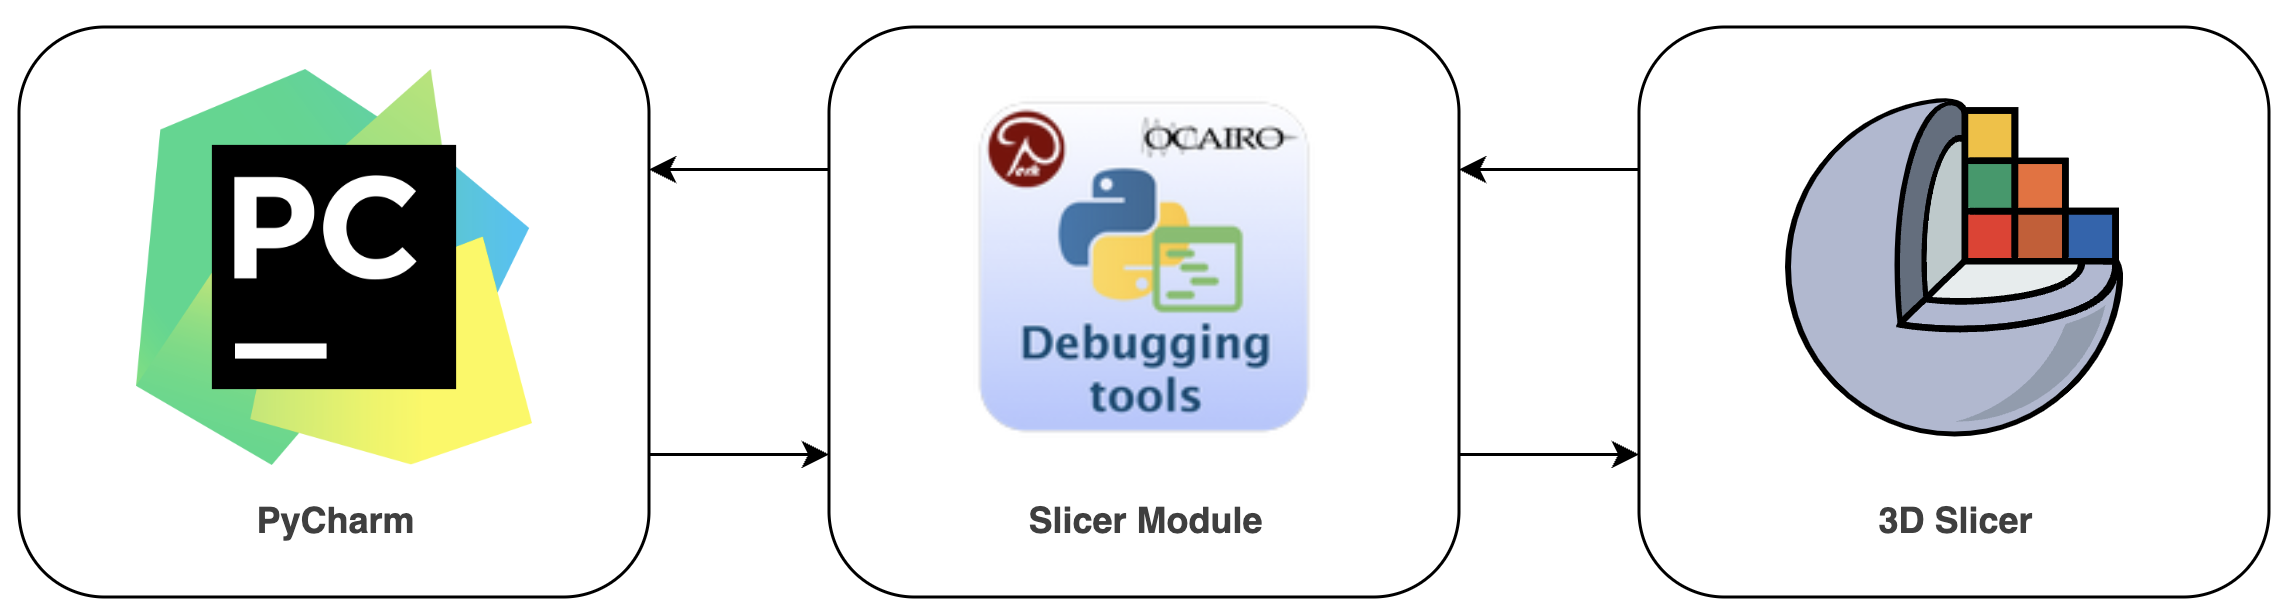
\includegraphics[width=0.6\textwidth]{img/Entwicklungsumgebung.png}
	\caption{Umgebung während der Entwicklung mit 3D Slicer und PyCharm}
	\label{fig:entwicklungsumgebung}
\end{figure}

Mit dem Debugging Tool lässt sich eine gewohnte Umgebung reproduzieren, in der
der Quellcode Schritt für Schritt analysiert werden kann \citep[vgl.][]{slicerdebuggingtools}.
Speziell bei der Fehlersuche ist dieses Tool eine sehr gute Unterstützung. Die Abbildung
beschreibt weiter, das als Umgebung für das Erstellen des Programmcodes die
Software Pycharm verwendet wird. Pycharm ist eine Lösung der Firma Jetbrains,
für das Erstellen von Python-Quellcode. Dieses Tool bietet eine breite Palette an
Funktionalitäten, die das Erstellen von Software vereinfachen und als \textit{State
of the Art} bezeichnet werden kann \citep[vgl.][]{jetbrains2024}.

Damit während der Entwicklung auch Teilbereiche der Software bereits getestet
werden können, werden Testdaten benötigt. Bei diesen Testdaten handelt es sich
um originale Mikro-\ac{CT}-Aufnahmen von Zahnstrukturen. Diese wurden auf einem
Server an der \ac{LMU} in München bereitgestellt und konnten über den \textit{x2goclient}
heruntergeladen werden. Mit dem Zugriff auf den Galadriel-Rechner an der \ac{LMU}
konnten auch diverse Pythonumgebungen zum Verarbeiten von Daten genutzt werden. Dies
war in erster Linie für ein Nachvollziehen der anatomischen Segmentierung hilfreich.

Neben der eigentlichen Umgebung und den Entwicklerwerkzeugen steht zur Entwicklung
auch ein Python Paket zur Verfügung, das von Herrn Prof. Rösch speziell für die Klinik
an der \ac{LMU} erstellt wurde. Dieses Tool beinhaltet diverse Funktionalität für
das Verarbeiten von medizinischen Bilddaten. Speziell für die Mikro-\ac{CT}-Aufnahmen
der Klinik. Für die Interaktion mit der Slicer Kernanwendung stellt der Python-Interpreter
das Paket \texttt{slicer} zur Verfügung. Hierdurch lassen sich diverse
Mechanismen steuern. Wichtig ist hierbe, dass das Paket \texttt{slicer} nicht auf
\ac{PyPi} zu finden ist.

Nachdem die Anforderungen, die Recherche, die konkreten Aufgaben und die
verfügbaren Werkzeuge erläutert wurden, bleibt noch die Evaluation der Arbeit.
Das Kapitel Forschungsevaluation erläutert die Methodik, mit dem das Erreichen des
Forschungsziels messbar gemacht werden kann.

% ---------------------------------------------------------------------------------------

\section{Forschungsevaluation}
Die Evaluation kann grob in zwei Teile unterteilt werden. Der erste Teil ist der
wohl Wichtigste und beschäftigt sich mit dem Testen der Anwendung durch die Benutzer.
Hier kann also die Benutzerfreundlichkeit und die \ac{UI} der Erweiterung gut analysiert
werden. Dabei werden Verbesserungen gesammelt und als möglicher Ausblick zur
Verfügung gestellt. Wichtig für die Benutzbarkeit der Software ist auch das Benutzerhandbuch.
Dies ist auch Teil der Ergebnisse und muss mittels Benutzertests evaluiert
werden.

Der zweite Teil der Evaluation soll prüfen ob der softwaretechnische Ansatz
erfolgreich umgesetzt wurde. Um dies gewährleisten zu können, müssen zusätzlich
zur Funktionalität auch Softwaretests bereitgestellt werden. Wie eine der Teilaufgaben
aus Kapitel \ref{sec_zerlegung_in_teilprobleme} bereits zeigt, handelt es sich
hierbei um Unittests. Außerdem ist für diesen Teil auch die technische Dokumentation
notwendig. Abschießend soll die Performance des Systems noch gemessen und
analysiert werden.

Die in diesem Kapitel beschriebenen methodischen Schritte bildeten die Grundlage
für die Entwicklung der Erweiterung. Nachdem die Analysephase abgeschlossen ist,
folgen nun die Phasen Entwicklung und Evaluation in Form der Ergebnisse. Hierzu wird
die erstellte \ac{SEM} detalliert vorgestellt und die Funktionen näher
beschrieben.
% ---------------------------------------------------------------------------------------